\documentclass[%
	%draft, %submission,
	compressed,
	%final,
	% %technote,
	%internal,
	%submitted,
	%inpress,
	%reprint,
	%
	titlepage,
	%notitlepage,
	%anonymous,
	narroweqnarray,
	inline,
	twoside,
        %invited,
	]{ieee}

\usepackage[latin1]{inputenc}			% idioma
\usepackage[spanish]{babel}
\usepackage{color}
\usepackage{colortbl}
\usepackage{amsmath}
\usepackage{amsfonts}
\usepackage{verbatim}

% -------- PARA FIGURAS
\usepackage{graphicx}
\usepackage{capt-of}
% -------- FIN FIGURAS

\usepackage{hyperref}				% urls

% -------- PARA MOSTRAR EL CODIGO DE MANERA AMENA
\usepackage{courier}
\usepackage{listings}
\lstset{ %
	language=C++,                % choose the language of the code
	basicstyle=\footnotesize\ttfamily,       % the size of the fonts that are used for the code
	numbers=left,                   % where to put the line-numbers
	numberstyle=\footnotesize,      % the size of the fonts that are used for the line-numbers
	stepnumber=1,                   % the step between two line-numbers. If it is 1 each line will be numbered
	numbersep=5pt,                  % how far the line-numbers are from the code
	backgroundcolor=\color{white},  % choose the background color. You must add \usepackage{color}
	showspaces=false,               % show spaces adding particular underscores
	showstringspaces=false,         % underline spaces within strings
	showtabs=false,                 % show tabs within strings adding particular underscores
	frame=single,           % adds a frame around the code
	tabsize=6,          % sets default tabsize to 2 spaces
	captionpos=b,           % sets the caption-position to bottom
	breaklines=true,        % sets automatic line breaking
	breakatwhitespace=false,    % sets if automatic breaks should only happen at whitespace
}
% -------- FIN CODIGO

%\hypersetup{citecolor=black}	% color citas


%--------- PARA EL ENUNCIADO DE LA CATEDRA
\parskip = 11pt

%\addtolength{\hoffset}{-1cm}
%\addtolength{\textwidth}{2cm}
 \addtolength{\voffset}{-0.5cm}
 \addtolength{\textheight}{1cm}


\newcommand{\real}{\mathbb{R}}
\newcommand{\nat}{\mathbb{N}}
\newcommand{\eme}{\mathcal{M}}
\newcommand{\emeh}{\widehat{\mathcal{M}}}
\newcommand{\ere}{\mathcal{R}}
%----------- FIN PARA EL ENUNCIADO DE LA CATEDRA


\hypersetup{			%sacar los colores horrendos de las ref
	colorlinks=false,
	pdfborder={0 0 0},
}

\begin{document}


\title[Reconocimiento de d\'igitos manuscritos]{%
	Reconocimiento de d\'igitos manuscritos a partir de la factorizaci\'on SVD\\
{\small M\'etodos Num\'ericos, Departamento de Computaci\'on, Universidad de Buenos Aires}
}

\journal{M\'etodos Num\'ericos, Departamento de Computaci\'on, Universidad de Buenos Aires}
\author[ALEMAN, G. DIEZ Y SCOCCOLA]{
Guillermo Gallardo Diez\authorinfo{gagdiez.c@gmail.com},\and{}Damian Eliel Aleman\authorinfo{damianealeman@gmail.com},\and{}y Luis Scoccola\authorinfo{luis.scoccola@gmail.com}
}


\firstpage{1}

\maketitle               
\tableofcontents

\newpage

\begin{abstract} 
\end{abstract}

\begin{keywords}
\end{keywords}

%----------------------------------------------------------------------
\section{Introducc\'ion te\'orica}

\section{Introducc\'ion te\'orica}

\PARstart La factorizaci\'on SVD puede tener varias interpretaciones.
Se llama factorizaci\'on SVD de una matriz $A$ (de dimensiones arbitrarias)
a un producto de tres matrices $U\Sigma T^{t} = A$. Donde $U$ y $T$
son ortogonales y $Sigma$ tiene entradas nulas en todo elemento
$\sigma_{i,j}, i\neq j$ (usualmente llamada diagonal, si bien sus dimensiones
son iguales a las de $A$). Si las entradas de la diagonal de $\Sigma$ tienen
la particularidad de estar ordenadas de la forma $\sigma_{i,i} \geq
\sigma_{j,j}, i<j$, entonces esta factorizaci\'on es \'unica.

Esta factorizaci\'on puede ser interpretada de varias formas y suele
brindar mucha informaci\'on acerca de la matriz. En este caso queremos
calcular las componentes principales de un cierto vector que representa
una imagen de un d\'igito manuscrito.

Para esto usamos una base de datos de d\'igitos manuscritos.
Cada uno de estos d\'igitos es una imagen que la interpretamos como
un vector fila. De esta manera obtenemos una matriz de im\'agenes.
Donde la cantidad de columnas es la cantidad de pixeles en cada imagen
y la cantidad de filas es la cantidad de im\'genes.
A partir de esta base de datos nos interesa calcular la covarianza entre
cada pixel. Usamos la f\'ormula: JSDAKJSDBAD constrsdijnaskdjansjka

Las k-componentes principales de una imagen dada se obtienen ralizando
el producto interno entre el vector de la imagen y los k-autovectores
que se corresponden con los k-autovalores de mayor m\'odulo de la matriz
de covarianza.

 
%----------------------------------------------------------------------
\section{Desarrollo}

\section{Desarrollo}

\subsection{Descomposici\'on SVD}

	\PARstart De la introducci\'on se deduce que no es necesario calcular de forma
	completa toda la descomposici\'on en valores singulares. Basta tener
	las primeras $k$ columnas de $V$. Es decir necesitamos un m\'etodo para
	obtener los autovectores que se corresponden con los autovalores de mayor
	m\'odulo de una matriz.
	Es importante notar que la matriz con la que trabajamos es sim\'etrica
	con coeficientes reales y por lo tanto podremos utilizar metodos optimizados.
	Para obtener los autovectores implementamos dos estrategias:

	\begin{itemize}
		\item \textbf{M\'etodo de la Potencia y deflaci\'on:} Suponiendo que
		tenemos autovalores $\lambda_1\ \geq \ldots \geq |\lambda_n|$ y los primeros
		$k$ son distintos, obtenemos $\lambda_1$ (y su atovalor asociado),
		mediante el m\'etodo de la potencia. Luego
		construimos una matriz que tenga como autovalores
		$|\lambda_2| \geq \ldots \geq |\lambda_n| \geq 0$.
		De esta forma inductiva calculamos los primeros $k$ autovalores
		con sus correspondientes autovectores.

		\item \textbf{M\'etodo QR para matrices sim\'etricas tridiagonales y
		m\'etodo de la potencia inversa:} Asumiendo que partimos de una matriz
		sim\'etrica, obtenemos una matriz de hessemberg (y en este caso
		tridiagonal, por ser sim\'etrica) semejante, mediante reflexiones de
		Householder. Luego, mediante el algoritmo QR calculamos sus
		autovalores. Finalemente usamos esta aproximaci\'on de
		los autovalores para calcular los primeros $k$ autovectores con el m\'etodo
		de la potencia inversa.
	\end{itemize}

	A continuaci\'on se explican las implementaciones con m\'as detalle.

	\subsubsection{M\'etodo de la potencia y deflaci\'on}
		El m\'etodo de la potencia es un m\'etodo iterativo. Se parte con un vector
		inicial $v_0$ y se genera una sucesi\'on de vectores ${v_i}$ realizando,
		en cada iteraci\'on, $$v_{i+1} = \frac{Av_i}{\|Av_i\|_{\infty}}$$.
		Asumiendo que la matriz tiene un autovalor $\bar{\lambda}$ de m\'odulo
		estrictamente
		mayor al resto de los autovalores y que $v_0$ no es ortogonal al
		autovector $\bar{v}$ asociado a dicho autovalor, la sucesi\'on converge 
		a $\bar{v}$.

		El metodo no depende fuertemente de la norma que se usa para renormalizar
		en cada iteraci\'on. La \'unica diferencia es que el autovector obtenido
		estar\'a normalizado con la norma usada. En nuestro caso usamos la norma
		infinito porque se calcula de manera m\'as rapida.

		Una vez que tenemos el autovalor $\bar{\lambda}$ obtenemos una matriz
		$A'$ que conserva los mismos autovalores y autovectores exceptuando
		$\bar{\lambda}$ y $\bar{v}$, realizando:
		$$A' = A-\bar{\lambda}\bar{v}\bar{v}^t$$

	\subsubsection{M\'etodo QR para matrices sim\'etricas tridiagonales y m\'etodo
	de la potencia inversa}

		Como la matriz de covarianza es sim\'etrica. Utilizamos el algoritmo
		$9.5$ de \cite{burden} para obtener una matriz tridiagonal semejante a \'esta.
		Esta se obtiene mediante transformaciones de Householder.
		Una vez obtenida usamos el algoritmo $9.6$ para calcular sus autovalores.
		Dado que trabajamos con matrices tridiagonales los autovalores pueden
		calcularse r\'apidamente y con mucha precisi\'on.

		Luego utilizamos el m\'etodo inverso de la potencia.
		Este es bastante similar al m\'etodo de la potencia pero permite calcular
		cualquier par autovalor-autovector asumiendo las m\'ismas hip\'otesis
		que el m\'etodo de la potencia con el agregado de tener una aproximaci\'on
		razonable de los autovalores correspondientes a los autovectores que
		quieren calcularse.

		Partiendo de la matriz $A$ un autovector $v_0$ y una aproximaci\'on a un
		autovalor $\lambda$ obtenemos una sucesi\'on ${v_i}$ de autovectores
		que converge al autovector asociado al autovalor $\lambda$.
		Para esto planteamos la iteraci\'on:
		$$v_{i+1} = (A-\lambda Id)^{-1}v_i$$

		Notemos que este es el concepto matem\'atico. En nuestra implementaci\'on
		no invertimos la matriz, sino que resolvemos un sistema de ecuaciones
		en cada iteraci\'on. Para alivianar el tiempo de c\'omputo realizamos
		una descomposici\'on LU de la matriz del sistema que nos sirve para
		todas las iteraciones que se realicen con un mismo autovalor $\lambda$.

\subsection{Reconociendo d\'igitos usando las componentes principales}

	\PARstart Para reconocer d\'igitos a partir de sus componentes principales
	implementamos dos m\'etodos. Cada uno de los metodos puede ser usado con la
	cantididad de componentes principales que se desee y por lo tanto no se
	har\'a referencia a dicha cantidad en la explicaci\'on. En la parte test
	experimentaremos con diversas cantidad y buscaremos la m\'as adecuada para
	cada m\'etodo.

	\subsubsection{kVecinos}
		Se calculan las componentes principales $c$ de la imagen a evaluar
		y las componentes $c_i$ de todas las im\'agenes $x_i$ de las bases
		de datos. Se toman las distancias eucl\'ideas $\|c - c_i\|$
		y se cuentan las apariciones de cada d\'igito ($0, \ldots, 9$)
		en el conjunto de los $k$ $c_i$ m\'as cercanos a $c$.
		El d\'igito que registre mayor frecuencia se tomar\'a como el
		el d\'igito escrito en la imagen a evaluar.
	
	\subsubsection{kVecinos ponderados}
		En un principio pensamos calcular el promedio de las distancias $\|c - cj_i\|$.
		Donde $cj$ representa el conjunto de componentes principales de las
		im\'agenes del d\'igito $j$. De esta manera se est\'a tomando la 
		distancia promedio a todos los d\'igitos $1$, a los d\'igitos $2$, etc.

		Vimos que este metodo no daba resultados razonables y parametrizamos
		el mismo, para dar m\'as granularidad a la hora de utilizarlo.
		En lugar de promediar la distancia a todos los d\'igitos de la base
		de datos, lo hacemos \'unicamente con los $k$ d\'igitos que se
		encuentren m\'as cerca.
		
	\subsubsection{Distancia al promedio de las componentes}
		Para cada d\'igito $0, \ldots, 9$ se iteran todos los $c_i$ 
		y se generan diez $\bar{c}_j$ correspondientes con el
		promedio componente a componente de los $c_i$ de los
		d\'igitos $j$.
		Luego se calcula la distancia de $c$ a cada uno de los $\bar{c}_j$
		y se toma como d\'igito escrito al $j$ tal que $\|c - \bar{c}_j\|$
		sea m\'inimo.

\subsection{Tests}

	\subsubsection{Error de los autovectores calculados}
		Para los dos m\'etodos utilizados para calcular autovectores
		dise\~namos un experimento que busca cuantificar el error m\'aximo
		que tienen los resultados.
		Se calculan los primeros $k$ autovectores $v_i$ y se normalizan con la
		norma eucl\'idea. Luego se realiza $Av_i$ para cada $i$ y se normaliza
		el resultado, obteniendo $\hat{v}_i$. Finalmente se toman las diferencias
		$\|v_i-\hat{v}_i\|$. Mientras m\'as precisos sean los resultados del
		algoritmo, m\'as peque\~nas ser\'an estas distancias.
		De esta manera podemos comparar el comportamiento de los dos algoritmos
		con distintas tolerancias de entrada.
		
		Esperamos obtener resultados m\'as precisos al utilizar la estrategia
		\textit{QR-potencia Inversa}. Basamos esta hip\'otesis en que se usan
		matrices ortogonales para calcular los autovalores. Estas matrices
		tienen el n\'umero de condici\'on mas bajo posible, $1$.
		Una vez que tenemos aproximaciones de los autovalores de buena calidad
		el m\'etodo de la potencia inversa brinda buenas aproximaciones de los
		autovectores.

	\subsubsection{Diferencias en el tiempo de ejecuci\'on para obtener autovectores}
		Dado que ambos m\'etodos son esencialmente distintos cabe preguntarse
		si sus complejidades son distintas. Te\'oricamente notamos una diferencia
		importante: el m\'etodo de la potencia inversa resuelve un sistema de
		ecuaciones por cada autovector y por ende tiene una complejidad de $\Omega(n^3)$,
		donde $n$ representa la dimensi\'on de la matriz. Por otro lado el m\'etodo
		de la potencia solo realiza una multiplicaci\'on entre matriz y vector
		y por lo tanto tendr\'a una complejidad de $\Omega(n^2)$.

		Por este motivo esperamos ver una diferencia significativa en el tiempo de
		ejecuci\'on de ambas estrategias.

	\subsubsection{Cantidad de d\'igitos reconocidos en funci\'on de el m\'etodo,
	la cantidad de componentes utilizada y la precisi\'on de los autovectores}
		Comenzamos buscando buenos par\'ametros para los m\'etodos de reconocimiento
		de d\'igitos. Para esto calculamos autovectores con la mejor precisi\'on
		posible y experimentamos con la cantidad de componentes entre $20$ y $100$.
		Una vez que obtenemos los par\'ametros que se comportan mejor para cada
		m\'etodo analizamos la diferencia de comporamiento de los m\'etodos
		al variar la cantidad de componentes principales y la precisi\'on con
		la cual se calculan los autovectores.

	\subsubsection{Influencia del tama\~no de la base de datos}
		Bas\'andonos en el test anterior comparamos el \textit{hit rate} logrado
		por los m\'etodos de reconocimiento de d\'igitos al variar al cantidad
		de im\'agenes en la base de datos.
		
	\subsubsection{D\'igitos mejor reconocidos en funci\'on del m\'etodo}
		Dado que implementamos m\'as de un m\'etodo para el reconocimiento de
		d\'igitos, nos preguntamos si los mismos funcionan mejor en distintos
		d\'igitos. Para responder al interrogante calculamos el \textit{hit rate}
		de cada d\'igito por separado y comparamos los resultados de los
		distintos m\'etodos.

\PARstart Testeamos los algoritmos en tres etapas.

\subsection{Efectos en la se\~nal y el espectro}

Graficamos el espectro original y el filtrado para se\~nales
de audio.
La idea, es mostrar que, por m\'as que ganemos
cierto rango din\'amico, no estaremos filtrando el ruido en
si, sino frecuencias que lo hacen m\'as notable.

\subsection{Buenos par\'ametros para se\~nales espec\'ificas}

Tomando un conjunto de audios e im\'agenes buscamos par\'ametros
de ambos filtros que maximicen el rango din\'amico ganado para
distintos niveles de ruido agregado.
Queremos ver cuando los filtros resultan m\'as efectivos.
Es decir, si lo son en la presencia de m\'as o menos ruido.

\subsection{Tiempo de corrida}

Para el caso de las im\'agenes comparamos el tiempo de ejecuci\'on
de los filtros est\'andar con los filtros por bloques para
distintos tama\~nos de bloque. Esperamos ver una complejidad
cuadr\'atica para bloques peque\~nos e imagenes grandes
ya que las operaciones de resoluci\'on de sistemas ser\'an
despreciables y se notar\'a m\'as que nada el recorrido de la matriz
principal, de tama\~no cuadr\'atico en funci\'on del lado.


%----------------------------------------------------------------------
\section{Resultados}

\section{Resultados}

	\subsubsection{Error de los autovectores calculados}
		
	\subsubsection{Diferencias en el tiempo de ejecuci\'on para obtener autovectores}
		

	\subsubsection{Cantidad de d\'igitos reconocidos en funci\'on de el m\'etodo,
	la cantidad de componentes utilizada y la precisi\'on de los autovectores}
		


	\subsubsection{Influencia del tama\~no de la base de datos}

	\subsubsection{D\'igitos mejor reconocidos en funci\'on del m\'etodo}


%----------------------------------------------------------------------
\section{Discusi\'on}

\section{Discusi\'on}

	\PARstart A continuaci\'on discutimos cada uno de los resultados obtenidos en los tests
	realizados.

	\subsection{Error de los autovectores calculados}

		No nos result\'o sencillo interpretar los resultados. Esperabamos ver una
		variaci\'on m\'as significativa en las distancias. Deducimos que las instancias
		que manejamos tienen una influencia en estos resultados:
		se trata de matrices de covarianza con coeficientes realmente grandes (del orden
		de $10^4$ y m\'as). Adem\'as las matrices son considerablemente esparsas ya que
		las im\'agenes de los d\'igitos suelen contener muchos ceros, pues se trata de
		lineas sobre fondo blanco.
		Considerando lo anterior nos result\'o razonable usar una tolerancia de $0.001$
		para obtener resultados \'optimos en el caso del m\'etodo de la potencia.

		Con respecto al m\'etodo \textit{QR-potencia Inversa} llegamos a la conclusi\'on
		de que tolerancias de estos \'ordenes no tiene influencia pr\'actica en los resultados.
		Esto se debe a que el m\'etodo comienza buscando una matriz semejante que sea
		tridiagonal. Una vez obtenida esta matriz verificamos que los elementos de la diagonal
		suelen ser alg\'un orden de magnitud m\'as grandes que los de la sub-diagonal.
		Tengamos en cuenta que hasta este punto no se utiliz\'o la tolerancia ya que
		obtener la matriz de hessemberg es un m\'etodo determinista, en el sentido de que
		lleva una cantidad de pasos bien definida (que depende del tama\~no de la matriz).
		No se trata de un m\'etodo iterativo.

		Teniendo una diferencia realmente grande entre diagonal y sub-diagonal, al m\'etodo QR,
		no le toma m\'as que unas pocas iteraciones converger. En este momento la tolerancia
		entra en juego. Pero la convergencia del m\'etodo es muy r\'apida y por ende habr\'a
		muy pocas iteraciones de diferencia para dos tolerancias significativamente distintas.

		Al tener autovalores calculados con una muy buena precisi\'on, el m\'etodo de la
		potencia inversa converge casi instantaneamente\footnote{Comprobamos que no suele tomar
		m\'as de dos iteraciones. En la discusi\'on del pr\'oximo experimento se hace evidente
		que la cantidad de iteraciones que le lleva converger no depende significativamente
		de la tolerancia utilizada.}. Esto se debe a que resuelve un sistema de ecuaciones
		utilizamndo una aproximaci\'on buena de los autovalores. Al utilizar la descomposici\'on
		LU para resolver el sistema buscamos mantener el error lo m\'as acotado posible.
		Suponemos que esto es efectivo al menos en estas instancias, pues, como afirmamos
		en la secci\'on \textbf{Resultados}, el error de los autovectores es realmente
		insigificante para toda tolerancia razonable.
		
	\subsection{Diferencias en el tiempo de ejecuci\'on para obtener autovectores}

		Notamos que, como da a entender el experimento anterior, la velocidad de convergencia
		del m\'etodo \textit{QR-potencia Inversa} no depende fuertemente de la precisi\'on
		utilizada. Por el contrario el m\'etodo de la potencia parece mostrar un comportamiento
		lineal en la precisi\'on. Esto es avalado por la teor\'ia, ya que el m\'etodo de la
		potencia tiene, te\'oricamente, una convergencia lineal.

		Estos resultados cumplen con nuestras expectativas, ya que el m\'etodo \textit{QR-potencia
		Inversa} toma un tiempo de circa un orden de magnitud m\'as que el m\'etodo de la potencia.

	\subsection{Cantidad de d\'igitos reconocidos en funci\'on del m\'etodo,
	cantidad de componentes utilizada y la precisi\'on de los autovectores}
		
		Para el m\'etodo de los vecinos ponderados encontramos que la catitdad \'optima de
		vecinos es $1$. Esto muestra que el m\'etodo no es realmente efectivo, ya que,
		para un solo vecino es equivalente al m\'etodo de los vecinos est\'andar.
		Por este motivo concluimos que el metodo no es \'util.

		El m\'etodo de los vecinos est\'andar mostr\'o un mejor comportamiento al
		usar $5$ vecinos. Esto concuerda con resultados discutidos con nuestros
		compa\~nero de clase. Para el resto de los test utilizamos esta cantidad
		de vecinos.

		Para el m\'etodo de los vecinos encontramos que una buena cantidad de componentes
		principales a utilizar es $50$.
		Como deducimos del primer test no notamos una diferencia importante en el \textit{hit rate}
		cuando se var\'ia la tolerancia usando el m\'etodo de la potencia. Notamos una variaci\'on
		de $\sim 0.2\%$ al cambiar la precisi\'on. Con lo cual nos convencemos de que, utilizando
		el m\'etodo de la potencia, una tolerancia del \'orden de $0.001$ es suficiente para
		conseguir resultados \'optimos.
		Por otro lado, es importante notar que la calidad de los resultados del m\'etodo de los
		vecinos depende m\'as de la cantidad de componentes usada que de la cantidad de vecinos.

		Finalmente analizamos el m\'etodo de la distancia al promedio de las componentes
		principales. Si bien el m\'etodo es computacionalmente m\'as simple, ya que se
		compara cada d\'igito a reconocer \'unicamente con diez promedios, no muestra
		resultados satisfactorios, apenas logra superar el $70\%$ de \textit{hits}.
		Notamos que para un comportamiento \'optimo necesita del orden de la mitad de
		componentes principales que el m\'etodo de los vecinos, con lo cual el m\'etodo
		funciona mucho m\'as r\'apido.


	\subsection{Cantidad de d\'igitos reconocidos en funci\'on del m\'etodo,
	cantidad de componentes utilizada y la precisi\'on de los autovectores}

		Vemos que el tama\~no del \textit{training set} determina el porcentaje de d\'igitos bien
		reconocidos en todos los casos. Pero la diferencia no es abismal. Utilizando una instancia
		diez veces m\'as grande logramos una mejora de circa $5\%$.

		Aqu\'i tambi\'en se pone en evidencia que la diferencia de precisi\'on entre el m\'etodo
		\textit{QR-potencia Inversa} y el \textit{pontencia-deflaci\'on} no implica resultados
		demasiado distintos.

	\subsection{D\'igitos mejor reconocidos en funci\'on del m\'etodo}

		Aqu\'i se nota bien la diferencia entre los dos m\'etodos de reconocimiento de
		d\'igitos. El m\'etodo de los vecinos tiene un comportamiento casi perfecto en
		los d\'igitos $0$ y $1$, y para cualquier otro d\'igito no baja del $90\%$ de
		\textit{hits}. Por el contrario, el m\'etodo de la distancia al promedio de las
		componentes es mucho m\'as inestable. Por ejemplo vemos que con el $4$ y el $5$
		tiene un \textit{hitrate} por debajo del $50$. Este tipo de analisis puede ayudar
		a desarrollar software m\'as inteligente: sabiendo en cuales d\'igitos es efectivo
		cada m\'etodo, pueden usarse varios m\'etodos simultaneamente, y tomar una decisi\'on
		en funcion del \textit{guess} de los distintos m\'etodos.


%----------------------------------------------------------------------
\section{Conclusiones}

\section{Conclusiones}

	\PARstart Analizamos dos m\'etodos de c\'alculo de autovectores y dos (efectivos)
	de reconocimiento de d\'igitos.

	Para los autovectores el m\'etodo m\'as preciso result\'o el
	\textit{QR-potencia Inversa}. Comprobamos que los autovectores suelen
	ser muy precisos, ya que su direcci\'on no se ve pr\'acticamente alterada
	por multiplicarlos por la matriz. El m\'etodo se comporta muy bien para
	tolerancias relativamente grandes (en el tipo de matrices que analizamos)
	y no suele depender fuertemente de la tolerancia elegida. Por otro lado
	no es un m\'etodo particularmente r\'apido, y, si se admite un poco de
	error, pueden obtenerse resultados razonables bastante m\'as rapido
	con el m\'etodo \textit{potencia-deflaci\'on}. Para este caso particular
	notamos una diferencia en los resultados obtenidos al comparar los
	dos m\'etodos de obtenci\'on de autovectores. Pero las diferencias
	pueden considerarse tolerables ya son del \'orden de $\sim 0.5\%$ de \textit{hit rate} para
	ambos m\'etodos de reconocimiento de d\'igitos.

	Con respecto al reconocimiento de d\'igitos creemos que el m\'etodo del
	promedio (al menos nuestra implementaci\'on) no es suficientemente buena
	para ninguna aplicaci\'on pr\'actica. En el mejor caso obtuvimos un
	\textit{hit rate} del $\sim 71\%$. A lo sumo puede combinarse con un m\'etodo
	tam\'as poderoso (como el de los vecinos) para hacer un \textit{double check}
	en el caso en el que el de los vecinos no llegue a un resultado concluyente
	\footnote{Por ejemplo, si los vecinos contienen cantidades similares
	de d\'igitos $a$ y d\'igitos $b$, $a\neq b$.}.
	El m\'etodo de los vecinos result\'o ser muy satisfactorio. Su mayor
	deficiencia est\'a en los d\'igitos $8$ y $9$ como mostramos en el \'ultimo
	test.


	De los resultados concluimos que el par\'ametro m\'as sensible
	para tener un bien \textit{hit rate} es la cantidad de componentes principales utilizadas
	pues, tanto la precisi\'on de los autovectores, como la cantidad de vecinos
	del m\'etodo de los vecinos, influyen de manera mucho menos notable
	en la cantidad de d\'igitos acertados.

	LO MAS IMPORATNE ES LA CANTIDAD DE COMPONENTES Y NO LOS ECINOS NI LA PRECISION


%----------------------------------------------------------------------

\begin{thebibliography}{1}

\bibitem{enunciado}
C\'atedra de M\'etodos num\'ericos,\\
\newblock {\em Tercer Trabajo Pr\'actico},\\
\newblock Primer cuatrimestre 2013

\end{thebibliography}

%----------------------------------------------------------------------

\newpage

\section{Ap\'endices}

\subsection{Enunciado}
\begin{centering}
\large\bf Laboratorio de M\'etodos Num\'ericos - Primer Cuatrimestre 2013 \\
\large\bf Trabajo Pr\'actico N\'umero 3: OCR+SVD\\
\end{centering}


\vskip 0.5 cm
\hrule
\vskip 0.1 cm

{\bf Introducci\'on}

El reconocimiento \'optico de caracteres (OCR, por sus siglas en ingl\'es) es el proceso por el cual se traducen o convierten im\'agenes de d\'igitos o caracteres (sean \'estos manuscritos o de alguna tipograf\'ia especial) a un formato representable en nuestra computadora (por ejemplo, ASCII). Esta tarea puede ser m\'as sencilla (por ejemplo, cuando tratamos de determinar el texto escrito en una versi\'on escaneada a buena resoluci\'on de un libro) o tornarse casi imposible (recetas indescifrables de m\'edicos, algunos parciales manuscritos de alumnos de m\'etodos num\'ericos, etc).

El objetivo del trabajo pr\'actico es implementar un m\'etodo de reconocimiento de d\'igitos manuscritos basado en la descomposici\'on en valores singulares, y analizar emp\'iricamente los par\'ametros principales del m\'etodo.

Como instancias de entrenamiento, se tiene un conjunto de $n$ im\'agenes de d\'igitos ma\-nus\-cri\-tos en escala de grises del mismo tama\~no y resoluci\'on (varias im\'agenes de cada d\'igito). Cada una de estas im\'agenes sabemos a qu\'e d\'igito se corresponde.
En este trabajo consideraremos la popular base de datos MNIST, utilizada como referencia en esta \'area de investigaci\'on\footnote{\texttt{http://yann.lecun.com/exdb/mnist/}}. 

Para $i = 1,\ldots, n$, sea $x_i \in \real^{m}$ la $i$-\'esima imagen de nuestra base de datos almacenada por filas en un vector, y sea $\mu = (x_1 + \ldots + x_n)/n$ el promedio de las im\'agenes. Definimos $X\in\real^{n\times m}$ como la matriz que contiene en la $i$-\'esima fila al vector $(x_i - \mu)^{t}/\sqrt{n-1}$, y $$X=U \Sigma V^t$$ a su descomposici\'on en valores singulares, con $U\in\real^{n\times n}$ y $V\in\real^{m\times m}$ matrices ortogonales, y $\Sigma\in\real^{n\times m}$ la matriz diagonal conteniendo en la posici\'on $(i,i)$ al $i$-\'esimo valor singular $\sigma_i$.
Siendo $v_i$ la columna $i$ de $V$, definimos para $i = 1,\ldots,n$ la \textsl{transformaci\'on caracter\'istica} del d\'igito $x_{i}$ como el vector $\mathbf{tc}(x_i) = (v_1^t\, x_i, v_2^t\, x_i,\ldots,v_k^t\, x_i) \in\real^k$, donde $k \in\{1,\ldots,m\}$ es un par\'ametro de la implementaci\'on. Este proceso corresponde a extraer las $k$ primeras \textit{componentes principales} de cada imagen. La intenci\'on es que $\mathbf{tc}(x_i)$ resuma la informaci\'on m\'as relevante de la imagen, descartando los detalles o las zonas que no aportan rasgos distintivos.


Dada una nueva imagen $x$ de un d\'igito manuscrito, que no se encuentra en el conjunto inicial de im\'agenes de entrenamiento, el problema de reconocimiento consiste en determinar a qu\'e d\'igito corresponde. Para esto, se calcula $\mathbf{tc}(x)$ y se compara con $\mathbf{tc}(x_i)$, para $i = 1,\ldots, n$.


{\bf Enunciado}

Se pide implementar un programa que lea desde archivos las im\'agenes de entrenamiento de distintos d\'igitos manuscritos y que, utilizando la descomposici\'on en valores singulares, se calcule la transformaci\'on caracter\'istica de acuerdo con la descripci\'on anterior. Para ello se deber\'a implementar alg\'un m\'etodo de estimaci\'on de autovalores/autovectores. Dada una nueva imagen de un d\'igito manuscrito, el programa deber\'a determinar a qu\'e d\'igito co\-rres\-pon\-de.
El formato de los archivos de entrada y salida queda a elecci\'on del grupo. Si no usan un entorno de desarrollo que incluya bibliotecas para la lectura de archivos de im\'agenes, sugerimos que utilicen im\'agenes en formato \textsc{Raw}. 


Se deber\'an realizar experimentos para medir la efectividad del reconocimiento, analizando tanto la influencia de la cantidad $k$ de componentes principales seleccionadas como la influencia de la precisi\'on en el c\'alculo de los autovalores.

\vskip 0.5 cm
\hrule
\vskip 0.1 cm

{\bf Fecha de entrega} 
\begin{itemize}
\item \textsl{Formato electr\'onico:} viernes 21 de junio de 2013, \underline{hasta las 23:59 hs.}, enviando el trabajo (informe+c\'odigo) a \texttt{metnum.lab@gmail.com}. El subject del email debe comenzar con el texto \verb|[TP3]| seguido de la lista de apellidos de los integrantes del grupo. 
\item \textsl{Formato f\'isico:} lunes 24 de junio de 2013, de 18 a 20hs (en la clase de la pr\'actica).
\end{itemize}


\newpage

\subsection{C\'odigo relevante}
\subsection{C\'odigo relevante y modo de uso}

	\subsubsection{Clase \textit{Reconocedor}}
		Esta clase permite utilizar cualquiera de los m\'etodos para el calculo
		de autovalores y combinarlo con cualquiera de los m\'etodo de reconocimiento
		de d\'igitos.
		
		\lstinputlisting{../../src_cpp/reconocedor.cpp}

	\subsubsection{Clase \textit{Matriz}}

		\lstinputlisting{../../src_cpp/matriz.h}


\newpage

\subsection{Tablas}
\subsubsection{Tabla A.}
    
    Promedio tiempo corrida m\'etodos:

    \vspace{5mm}
    \centerline{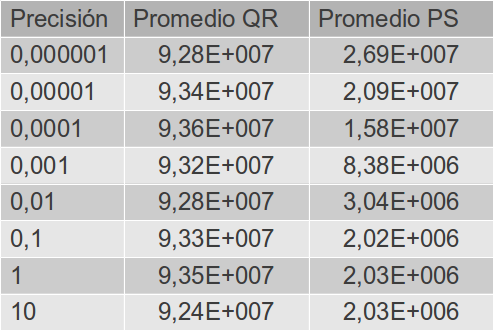
\includegraphics[width=7cm]{img/tiempoPromedio.png}}
    \vspace{5mm}

\subsubsection{Tabla B.}
    
    Porcentaje de digitos reconocidos Vecinos Ponderados:

    \vspace{5mm}
    \centerline{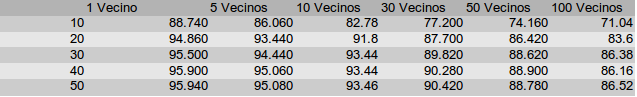
\includegraphics[width=14cm]{img/kVecinosPonderadosPs.png}}

\subsubsection{Tabla C.}
    
    Porcentaje de digitos reconocidos Vecinos:

    \vspace{5mm}
    \centerline{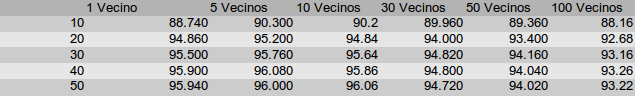
\includegraphics[width=14cm]{img/kVecinosPs.png}}

\subsubsection{Tabla D.}
    
    Cantidad de componentes con M\'etodo QR Potencia Inversa Kvecinos

    \vspace{5mm}
    \centerline{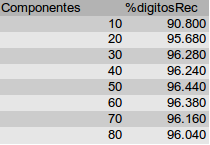
\includegraphics[width=4.5cm]{img/QrKvecinos.png}}


\subsubsection{Tabla E.}
    
    Cantidad de componentes con M\'etodo QR Potencia Simple Kvecinos

    \vspace{5mm}
    \centerline{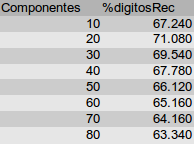
\includegraphics[width=4.5cm]{img/QRDigitosMEdios.png}}

\subsubsection{Tabla F.}
	
	Hitrate M\'etodos

	\vspace{5mm}
	\centerline{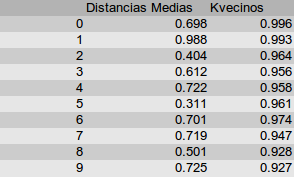
\includegraphics[width=7cm]{img/digitosBam_tabla.png}}



%----------------------------------------------------------------------

\end{document}
